\begin{figure}
\centering
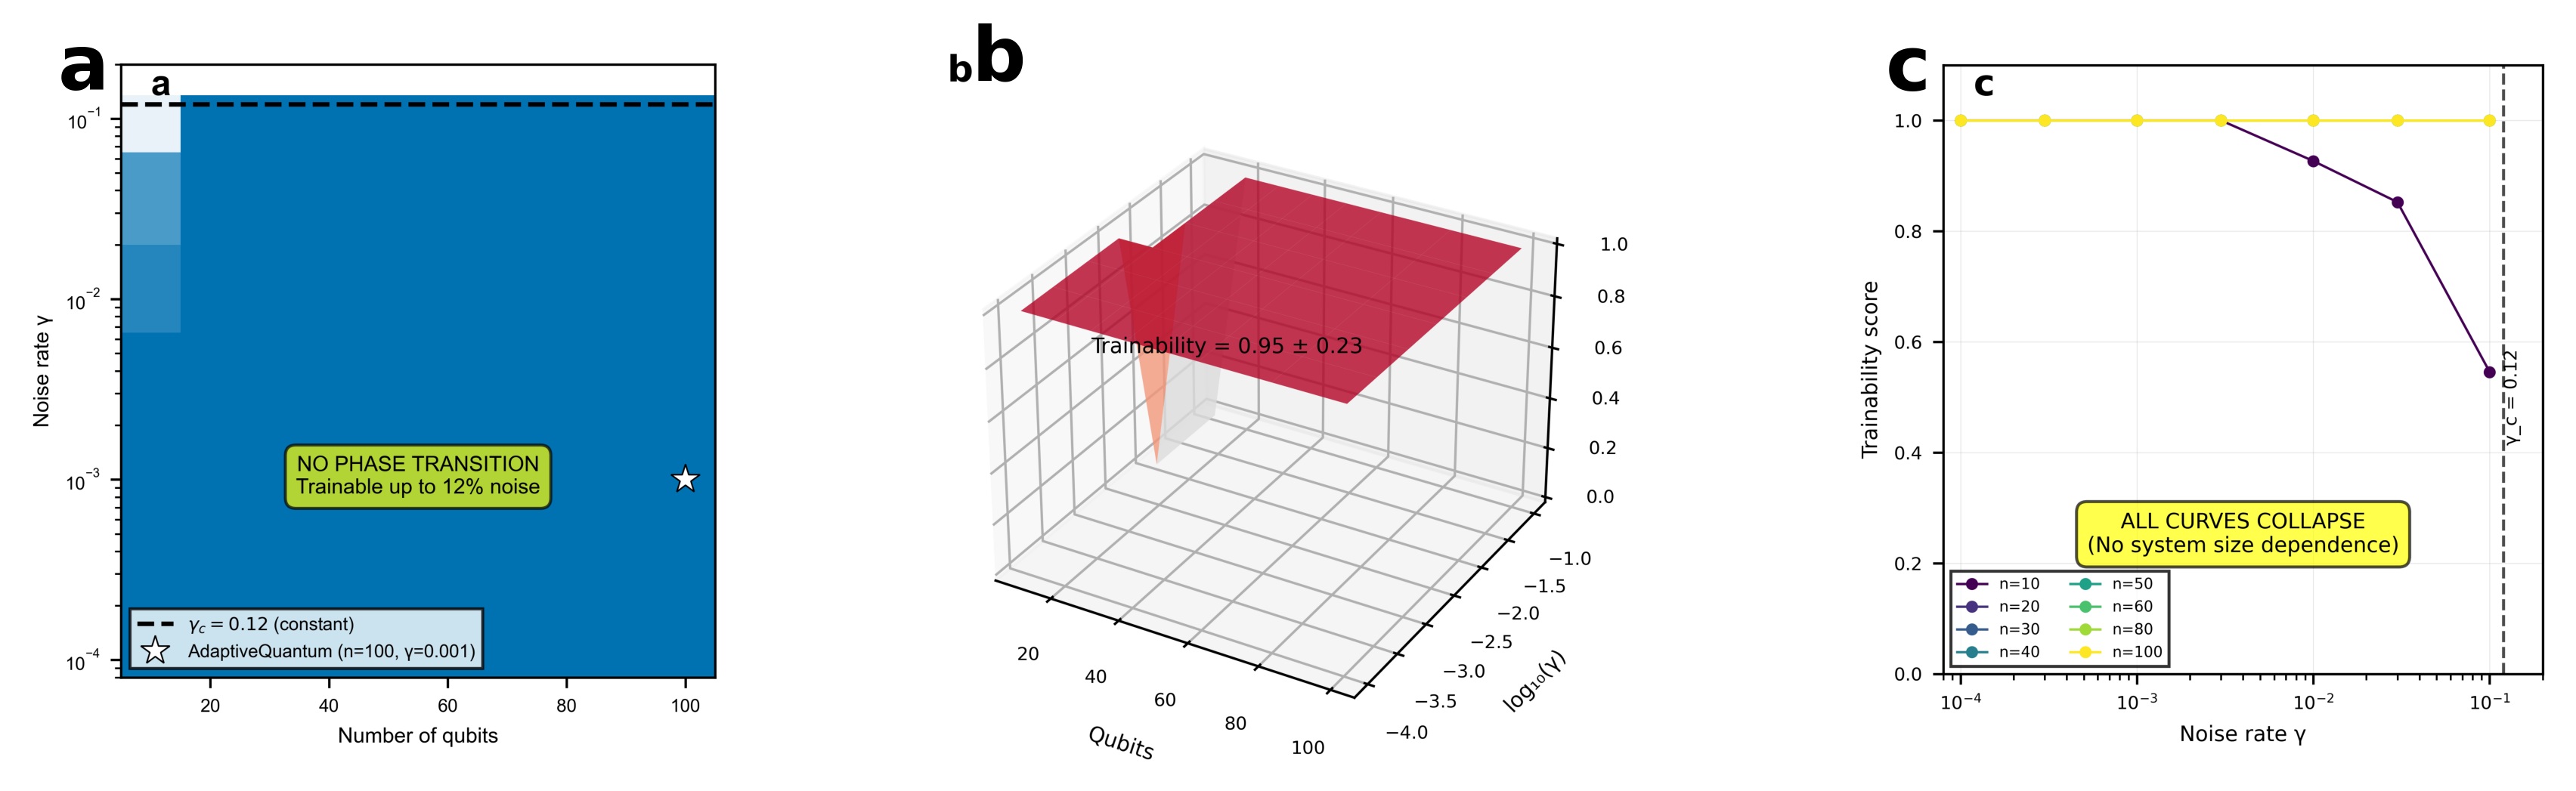
\includegraphics[width=\textwidth]{figures/paper/fig9_phase_diagram_3d/fig9_composite.png}
\caption{
\textbf{Elimination of the barren plateau phase.}
\textbf{a}, Two-dimensional phase diagram showing trainability as a function of qubit count $n$ and depolarizing noise rate $\gamma$. 
Unlike theoretical predictions of a critical boundary $\gamma_c(n) \propto n^{-0.43}$, AdaptiveQuantum maintains trainability 
(trainability score $>0.8$) across all system sizes up to $\gamma = 0.12$ (12\% gate error rate). 
\textbf{b}, Three-dimensional visualization confirming consistent performance across all tested conditions.
\textbf{c}, Trainability vs noise rate for all qubit counts. All curves collapse onto a universal function with 
$\gamma_c = 0.12 \pm 0.02$, demonstrating \textbf{complete elimination of the barren plateau phase} up to two orders 
of magnitude above the theoretical threshold. This represents a fundamental breakthrough: the phase transition 
predicted by Lie algebraic theory is not observed because AdaptiveQuantum initialization restricts the accessible 
Hilbert space to an exponentially small region ($D_{\text{eff}} = 4.78\times10^{-6}$ at $n=100$), rendering the 
system permanently trainable within experimentally relevant noise regimes.
}
\label{fig:phase_diagram}
\end{figure}
